\documentclass[draft]{agujournal2018}
\usepackage{apacite}
\usepackage{url}
\usepackage{lineno}
\usepackage{amsmath}
\usepackage{amssymb}
\linenumbers

\draftfalse

\journalname{JGR: Space Physics}

\begin{document}

%% ------------------------------------------------------------------------ %%
%
%  TITLE
%
%% ------------------------------------------------------------------------ %%

\title{Jovian Auroral Ion Precipitation: X-Ray Production from Oxygen and Sulfur Precipitation}

%% ------------------------------------------------------------------------ %%
%
%  AUTHORS AND AFFILIATIONS
%
%% ------------------------------------------------------------------------ %%

\authors{S. J. Houston\affil{1}, T. E. Cravens\affil{1}, D. R. Schultz\affil{2,3}, H. Gharibnejad\affil{2,4}, W. R. Dunn\affil{5}, D. K. Haggerty\affil{6}, A. M. Rymer\affil{6}, B. H. Mauk\affil{6}, G. R. Gladstone\affil{7}, N. Ozak\affil{8}}

\affiliation{1}{Department of Physics and Astronomy, University of Kansas, Lawrence, KS, USA}
\affiliation{2}{Department of Physics, University of North Texas, Denton, TX, USA}
\affiliation{3}{Now at Department of Physics and Astronomy, Northern Arizona University, Flagstaff, AZ, USA}
\affiliation{4}{Now at National Institute of Standards and Technology, Gaithersburg, MD, USA}
\affiliation{5}{Mullard Space Science Laboratory, University College London, London, UK}
\affiliation{6}{The Johns Hopkins University Applied Physics Laboratory, Laurel, Maryland, USA}
\affiliation{7}{Southwest Research Institute, San Antonio, Texas, USA}
\affiliation{8}{TBD}

%% Corresponding Author:
% Corresponding author mailing address and e-mail address:

\correspondingauthor{T. E. Cravens}{cravens@ku.edu}

%% Keypoints, final entry on title page.

%  List up to three key points (at least one is required)
%  Key Points summarize the main points and conclusions of the article
%  Each must be 100 characters or less with no special characters or punctuation

% Example:
% \begin{keypoints}
% \item	List up to three key points (at least one is required)
% \item	Key Points summarize the main points and conclusions of the article
% \item	Each must be 100 characters or less with no special characters or punctuation
% \end{keypoints}

\begin{keypoints}
\item Oxygen and sulfur precipitation into the jovian auroral atmosphere produce X-rays.
\item The Juno spacecraft has observed oxygen and sulfur precipitation above the polar caps.
\item Using Juno measurements, we are able to produce a significant number of X-rays.
\end{keypoints}

%% ------------------------------------------------------------------------ %%
%
%  ABSTRACT
%
% A good abstract will begin with a short description of the problem
% being addressed, briefly describe the new data or analyses, then
% briefly states the main conclusion(s) and how they are supported and
% uncertainties.
%% ------------------------------------------------------------------------ %%

%% \begin{abstract} starts the second page

\begin{abstract}
enter abstract here


enter abstract here


enter abstract here


enter abstract here


enter abstract here

\end{abstract}



%% ------------------------------------------------------------------------ %%
%
%  TEXT
%
%% ------------------------------------------------------------------------ %%

\section{Introduction}

X-ray production at Jupiter has been of interest to the space physics community from when it was first observed by the Einstein Observatory in April of 1979 \citep{metzger1983}.

Throughout this paper, following historical nomenclature, we will refer to the precipitating particle (either oxygen or sulfur) as an ion and the target particle (molecular hydrogen) as the atom, although the target particles often end up ionized and the precipitating particles can, and will, reach a neutral state.

\section{Physical Processes and Model Description}

The model presented in this manuscript is introduced in great detail by \citet{houston2018}, \citet{ozak2010}, \citet{ozak2013}, and the references therein.
\citet{houston2018} primarily focused on field-aligned currents (FAC) and ultraviolet (UV) emission from oxygen, \citet{ozak2010} showed X-ray production rates from precipitating oxygen and sulfur, and \citet{ozak2013} made predictions of FAC and airglow intensities that Juno would measure when it arrived to Jupiter.
We follow up on the promise of \citet{houston2018} to include energetic sulfur precipitation and oxygen improvements; however, proton precipitation will be left to a future publication. 

Here, we present X-ray productions from precipitating oxygen and sulfur, rather than FAC and UV emission.
We layout the differences and updates to the simulation, but the finer details of the model will be left to the previous papers.
Aside from optimization improvements, the main contrast can be summarized as follows:
\begin{itemize}
\item The Jovian atmosphere has been extended deeper, down below the 1 bar level.
\item Oxygen cross-sections previously only included non-simultaneous (NSIM) collisions; we now consider simultaneous (SIM) ion-target interactions.
\item Sulfur SIM cross-sections have now been analyzed and are included in the model.
\item X-ray opacity effects and efficiencies 
\item Juno data (both oxygen and sulfur measurements) are adapted and input into the simulation.
\end{itemize}

\subsection{Jovian Atmosphere}

\citet{houston2018} used a neutral atmosphere originally presented by \citet{maurellis2001} based on Galileo probe data \citep{seiff1996,seiff1997} and remote observations \citep{sada1998}.
The same atmosphere is used here, only we have extended the depth from 200 km to -88 km, where 0 km is set to where the pressure is equal to 1 bar (Fig. \ref{fig:atm}).
The deeper atmosphere has been generated using temperature-pressure profiles retrieved from NASA's Infrared Telescope Facility and the Texas Echelon Cross Echelle Spectrograph Instrument (IRTF-TEXES) \citep{sinclair2018} and the ideal gas law since the measurements come from below the homopause.

\begin{figure}[ht]
\centering
\includegraphics[width=\textwidth]{Figures/Atmosphere.eps}
\caption{Atmospheric density profiles of H$_{2}$, He, CH$_{4}$, and H based on data shown in \citet{maurellis2001} and \citet{sinclair2018}. Also shown is the neutral temperature profile as a function of altitude and pressure.}
\label{fig:atm}
\end{figure}

\subsection{Ion-Neutral Impact Processes}

\citet{houston2018} modeled oxygen precipitation using 9 different collision processes that occurred non-simultaneously as the ion precipitated through the atmosphere following the cross-section data presented by \citet{schultz2017} and summarized here:

\begin{subequations}
\begin{equation}
O^{q+} + H_{2} \rightarrow \begin{cases}
O^{q+} + H_{2}^{+} + e & \text{Single Ionization} \\
O^{q+} + 2H^{+} + 2e & \text{Double Ionization} 
\end{cases}
\label{eqn:ion}
\end{equation}
\vspace*{-0.5cm}

\begin{equation}
O^{q+} + H_{2} \rightarrow \begin{cases}
O^{(q-1)+}
\begin{cases}
H_{2}^{+} &  \text{Single Capture} \\
H^{+} + H^{+} + e &   \text{Transfer Ionization} \\
\end{cases} \\
\\
O^{(q-2)+}
\begin{cases}
2H^{+} \rightarrow O^{(q-1)+} + e & \text{Double Capture -- Autoionization} \\
H^{+} + H^{+} & \text{Double Capture} \\
\end{cases}
\end{cases}
\label{eqn:cap}
\end{equation}

\begin{equation}
O^{q+} + H_{2} \rightarrow \begin{cases}
O^{(q+1)} + H_{2}^{+} + 2e; H + H^{+} + 2e & \text{Single Stripping} \\
O^{(q+2)} + H_{2}^{+} + 3e; H + H^{+} + 3e & \text{Double Stripping} 
\end{cases}
\label{eqn:strip}
\end{equation}

\begin{equation}
O^{q+} + H_{2} \rightarrow
O^{q+} + H_{2}^{*}; H^{*} + H^{*} \hspace{.1in} \text{Electronic Excitation - All States}
\label{eqn:ex}
\end{equation}
\label{eqn:all}
\end{subequations}

However, since then, \citet{schultz2018} has proposed that target and projectile processes could occur simultaneously (referred to as SIM collisions) and the cross-sections should reflected this, ultimately providing the cross-sections for 35 processes that are used in the current model.
The NSIM and SIM projectile and target processes used are the following:

\begin{tabbing}
\= X$^{q+}$ + H$_2$ $\rightarrow$ X$^{q+}$ + H$_2^+$ + e;  X$^{q+}$ + H + H$^+$ + e \= $\;\;\;\;\;$ \= single ionization (SI) \\
\= X$^{q+}$ + H$_2$ $\rightarrow$ X$^{q+*}$ + H$_2^+$ + e;  X$^{q+*}$ + H + H$^+$ + e \= $\;\;\;\;\;$ \= SI + single projectile excitation (SI+SPEX) \\
\= X$^{q+}$ + H$_2$ $\rightarrow$ X$^{q+**}$ + H$_2^+$ + e;  X$^{q+**}$ + H + H$^+$ + e \= $\;\;\;\;\;$ \= SI + double projectile excitation (SI+DPEX) \\
\= X$^{q+}$ + H$_2$ $\rightarrow$ X$^{(q+1)+}$ + H$_2^+$ + 2e;  X$^{(q+1)+}$ + H + H$^+$ + 2e \= $\;\;\;\;\;$ \= SI + single stripping (SI+SS)\\
\= X$^{q+}$ + H$_2$ $\rightarrow$ X$^{(q+2)+}$ + H$_2^+$ + 3e;  X$^{(q+2)+}$ + H + H$^+$ + 3e \= $\;\;\;\;\;$ \= SI + double stripping (SI+DS) \\
\\
\> X$^{q+}$ + H$_2$ $\rightarrow$ X$^{q+}$ + H$^+$ + H$^+$ + 2e	 \>  \> double ionization (DI) \\
\> X$^{q+}$ + H$_2$ $\rightarrow$ X$^{q+*}$ + H$^+$ + H$^+$ + 2e \>  \> DI+SPEX \\
\> X$^{q+}$ + H$_2$ $\rightarrow$ X$^{q+**}$ + H$^+$ + H$^+$ + 2e \>  \> DI+DPEX \\
\> X$^{q+}$ + H$_2$ $\rightarrow$ X$^{(q+1)+}$ + H$^+$ + H$^+$ + 3e \>  \> DI+SS \\
\> X$^{q+}$ + H$_2$ $\rightarrow$ X$^{(q+2)+}$ + H$^+$ + H$^+$ + 4e	 \>  \> DI+DS \\
\\
\> X$^{q+}$ + H$_2$ $\rightarrow$ X$^{(q-1)+}$ + H$^+$ + H$^+$ + e  \>  \> transfer ionization (TI) \\
\> X$^{q+}$ + H$_2$ $\rightarrow$ X$^{(q-1)+*}$ + H$^+$ + H$^+$ + e  \>  \> TI+SPEX \\
\> X$^{q+}$ + H$_2$ $\rightarrow$ X$^{(q-1)+**}$ + H$^+$ + H$^+$ + e  \>  \> TI+DPEX \\
\> X$^{q+}$ + H$_2$ $\rightarrow$ X$^{q+}$ + H$^+$ + H$^+$ + 2e  \>  \> TI+SS \\
\> X$^{q+}$ + H$_2$ $\rightarrow$ X$^{(q+1)+}$ + H$^+$ + H$^+$ + 3e  \>  \> TI+DS \\
\\
\> X$^{q+}$ + H$_2$ $\rightarrow$ X$^{(q-2)+**}$ + H$^+$ + H$^+$ $\rightarrow$ X$^{(q-1)+}$ + e  \>  \> double capture autionization (DCAI) \\
\> X$^{q+}$ + H$_2$ $\rightarrow$ X$^{(q-2)+***}$ + H$^+$ + H$^+$ $\rightarrow$ X$^{(q-1)+*}$ + e  \>  \> DCAI+SPEX \\
\> X$^{q+}$ + H$_2$ $\rightarrow$ X$^{(q-2)+****}$ + H$^+$ + H$^+$ $\rightarrow$ X$^{(q-1)+**}$ + e  \>  \> DCAI+DPEX \\
\> X$^{q+}$ + H$_2$ $\rightarrow$ X$^{(q-2)+**}$ + H$^+$ + H$^+$ $\rightarrow$ X$^{q+}$ + 2e  \>  \> DCAI+SS \\
\> X$^{q+}$ + H$_2$ $\rightarrow$ X$^{(q-2)+**}$ + H$^+$ + H$^+$ $\rightarrow$ X$^{(q+1)+}$ + 3e  \>  \> DCAI+DS \\
\\
\> X$^{q+}$ + H$_2$ $\rightarrow$ X$^{(q-1)+}$ + H$_2^+$;  X$^{(q-1)+}$ + H + H$^+$ \> $\;\;\;\;\;$ \> single electron capture (SC) \\
\> X$^{q+}$ + H$_2$ $\rightarrow$ X$^{(q-1)+*}$ + H$_2^+$;  X$^{(q-1)+*}$ + H + H$^+$ \> $\;\;\;\;\;$ \> SC+SPEX \\
\> X$^{q+}$ + H$_2$ $\rightarrow$ X$^{(q-1)+**}$ + H$_2^+$;  X$^{(q-1)+**}$ + H + H$^+$ \> $\;\;\;\;\;$ \> SC+DPEX \\
\> X$^{q+}$ + H$_2$ $\rightarrow$ X$^{(q)+}$ + H$_2^+$ + e;  X$^{(q)+}$ + H + H$^+$ + e \> $\;\;\;\;\;$ \> SC+SS \\
\> X$^{q+}$ + H$_2$ $\rightarrow$ X$^{(q+1)+}$ + H$_2^+$ + 2e;  X$^{(q+1)+}$ + H + H$^+$ + 2e \> $\;\;\;\;\;$ \> SC+DS \\
\\
\> X$^{q+}$ + H$_2$ $\rightarrow$ X$^{(q-2)+}$ + H$^+$ + H$^+$ \> $\;\;\;\;\;$ \> double electron capture (DC) \\
\> X$^{q+}$ + H$_2$ $\rightarrow$ X$^{(q-2)+*}$ + H$^+$ + H$^+$ \> $\;\;\;\;\;$ \> DC+SPEX \\
\> X$^{q+}$ + H$_2$ $\rightarrow$ X$^{(q-2)+**}$ + H$^+$ + H$^+$ \> $\;\;\;\;\;$ \> DC+DPEX \\
\> X$^{q+}$ + H$_2$ $\rightarrow$ X$^{(q-1)+}$ + H$+$ + H$^+$ + e \> $\;\;\;\;\;$ \> DC+SS \\
\> X$^{q+}$ + H$_2$ $\rightarrow$ X$^{(q)+}$ + H$+$ + H$^+$ + 2e \> $\;\;\;\;\;$ \> DC+DS \\
\\
\> X$^{q+}$ + H$_2$ $\rightarrow$ X$^{q+}$ + H$_2^*$  \> \> target excitation (TEX) \\
\> X$^{q+}$ + H$_2$ $\rightarrow$ X$^{q+*}$ + H$_2^*$  \> \> TEX+SPEX \\
\> X$^{q+}$ + H$_2$ $\rightarrow$ X$^{q+**}$ + H$_2^*$  \> \> TEX+DPEX \\
\> X$^{q+}$ + H$_2$ $\rightarrow$ X$^{(q+1)+}$ + H$_2^*$ + e  \> \> TEX+SS \\
\> X$^{q+}$ + H$_2$ $\rightarrow$ X$^{(q+2)+}$ + H$_2^*$ + 2e \> \> TEX+DS
\end{tabbing}
where X stands for the projectile, either O or S. $q$ is the charge state and depends on the number of electrons bound to the ion; $q$ runs from 0 to 8 for O and from 0 to 16 for S.
Some processes are not possible for neutral or singly ionized atoms or, similarly, for fully stripped or O$^{7+}$ and S$^{15+}$ ions (e.g., for neutral O and S, SC and DC are not possible, or for O$^{8+}$ and S$^{16+}$, SS and DS are not considered).

The explicit calculation and implication to the stopping power that going from the NSIM to SIM cross-sections produces can be found in \citet{schultz2018}; but for the model presented, it has shifted the peaks of the charge state equilibrium fractions down to a lower initial ion energy, ultimately requiring less energy to fully strip both oxygen and sulfur ions.

\subsection{Charge State Equilibrium Fractions}

In a very broad sense, as an ion precipitates through the atmosphere each collision can result in four different outcomes for the projectile.
The ion can become excited (e.g. SPEX), become further ionized by losing an electron or two (e.g. DS), become less ionized by gaining an electron or two (e.g. DCAI), or nothing can happen to it while the collision solely affects the target (e.g. SI).
Each type of interaction is governed by the energy of the precipitating ion, a more energetic ion will generally be stripped of more electrons than one precipitating with less energy.
This can be shown by the charge state equilibrium fractions in figure \ref{fig:CSDoxy} for oxygen and figure \ref{fig:CSDsul} for sulfur.

\begin{figure}[ht]
\centering
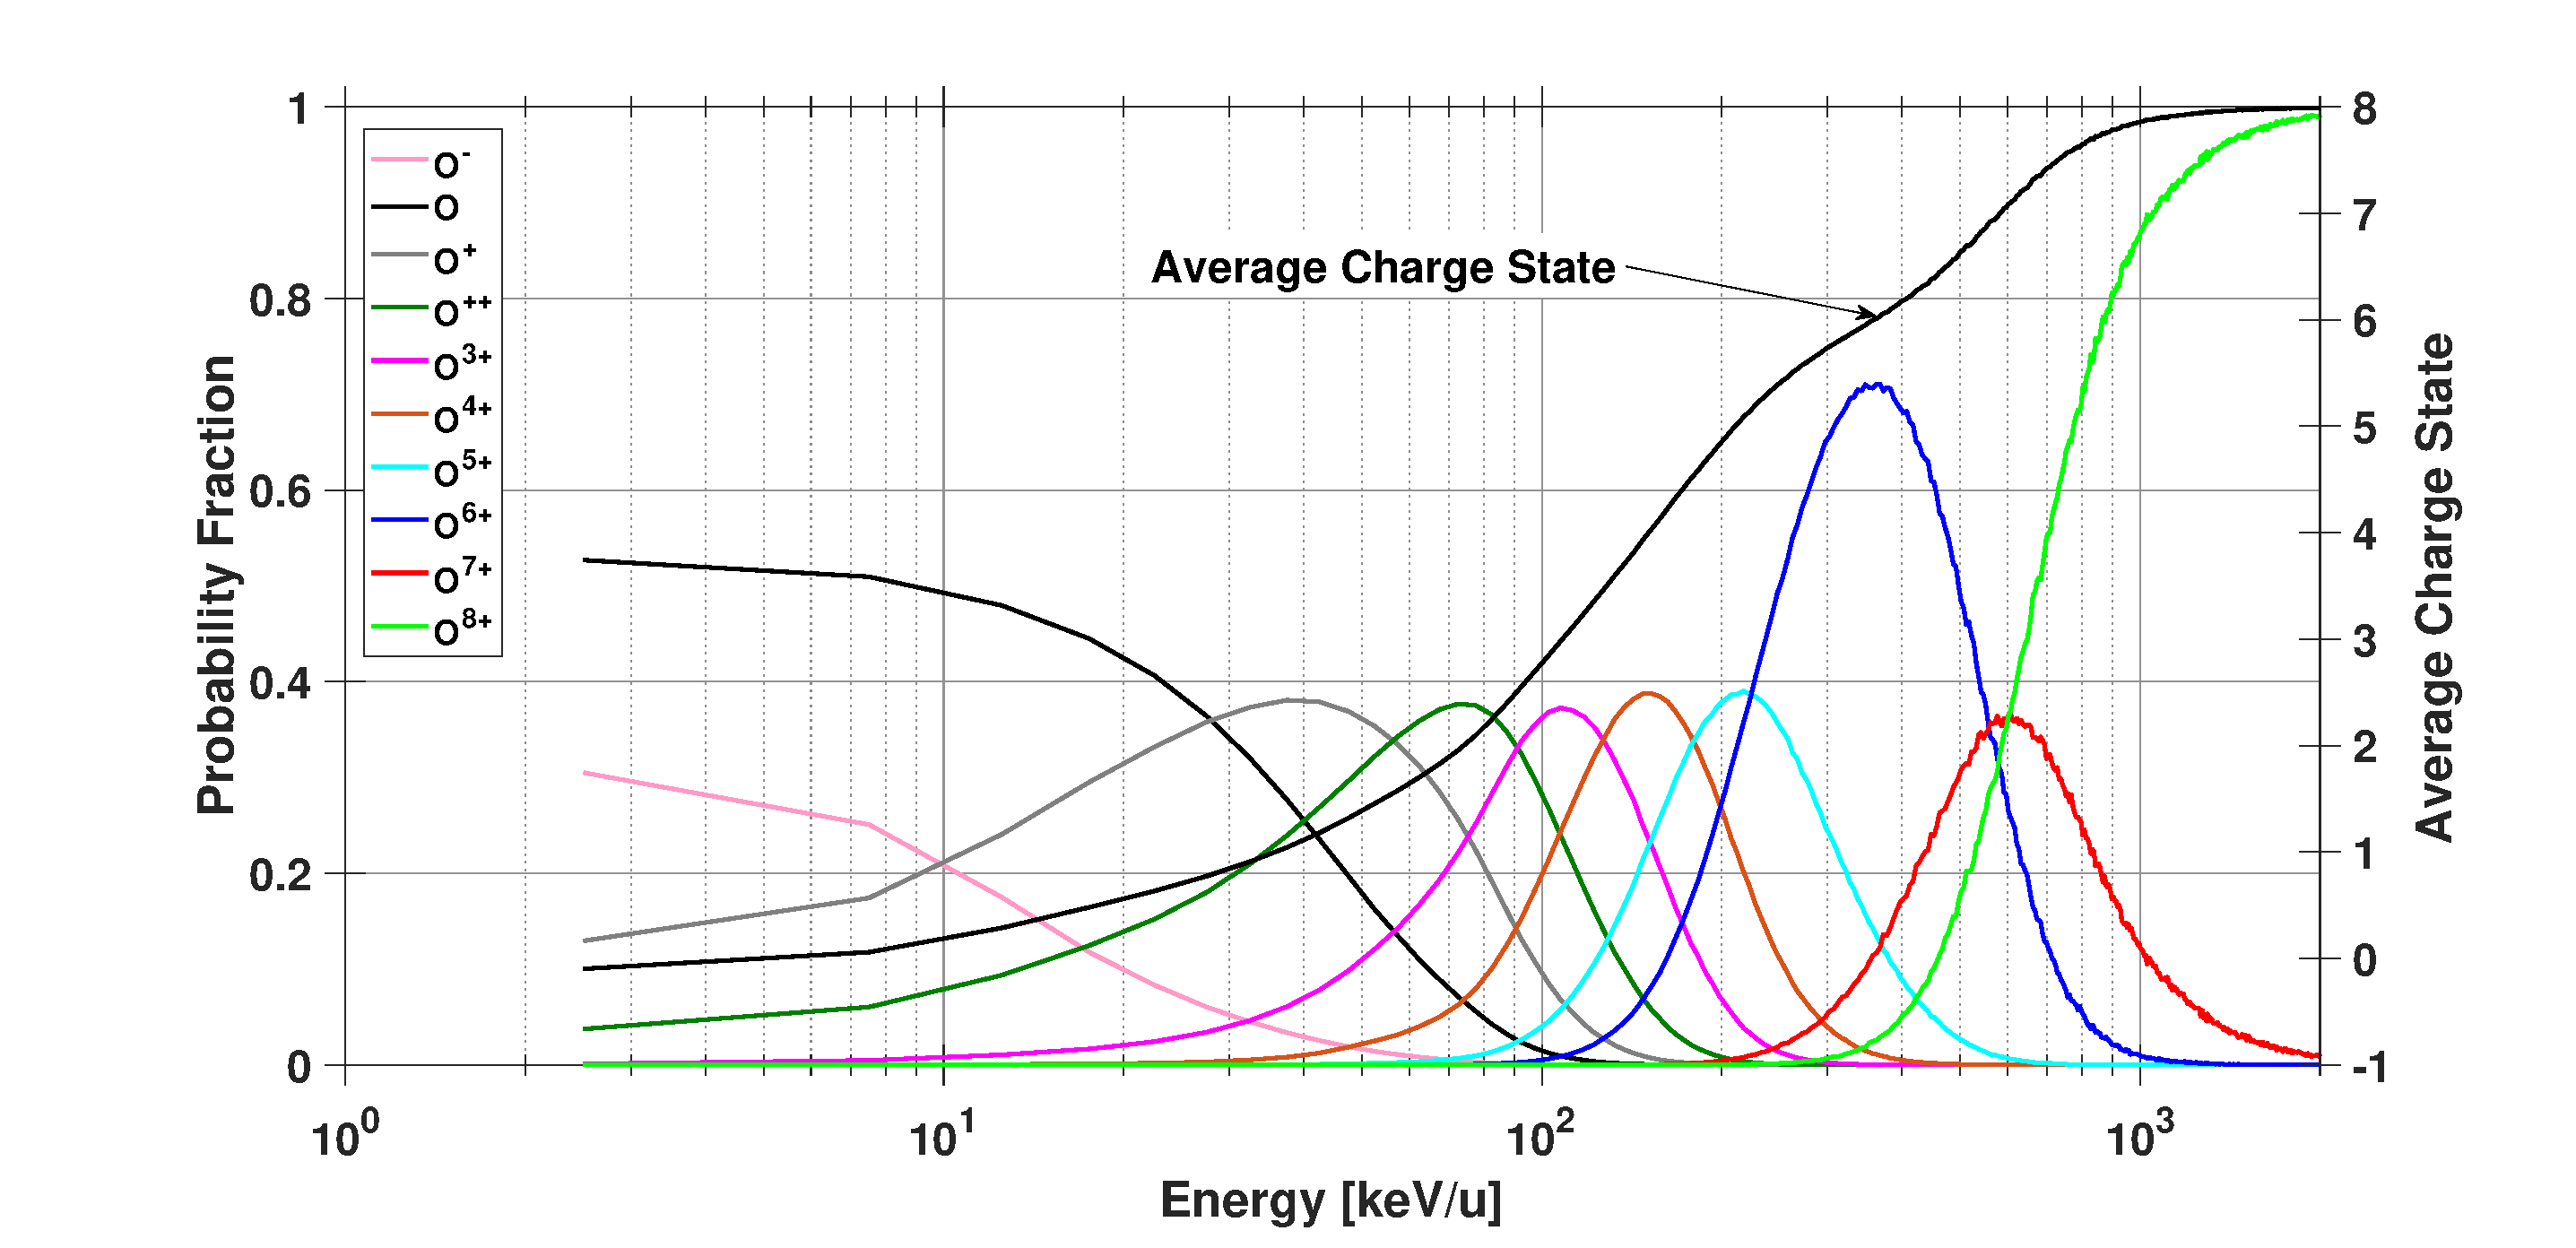
\includegraphics[width=\textwidth]{Figures/CSDoxy.eps}
\caption{Oxygen charge state distribution}
\label{fig:CSDoxy}
\end{figure}

\begin{figure}[ht]
\centering
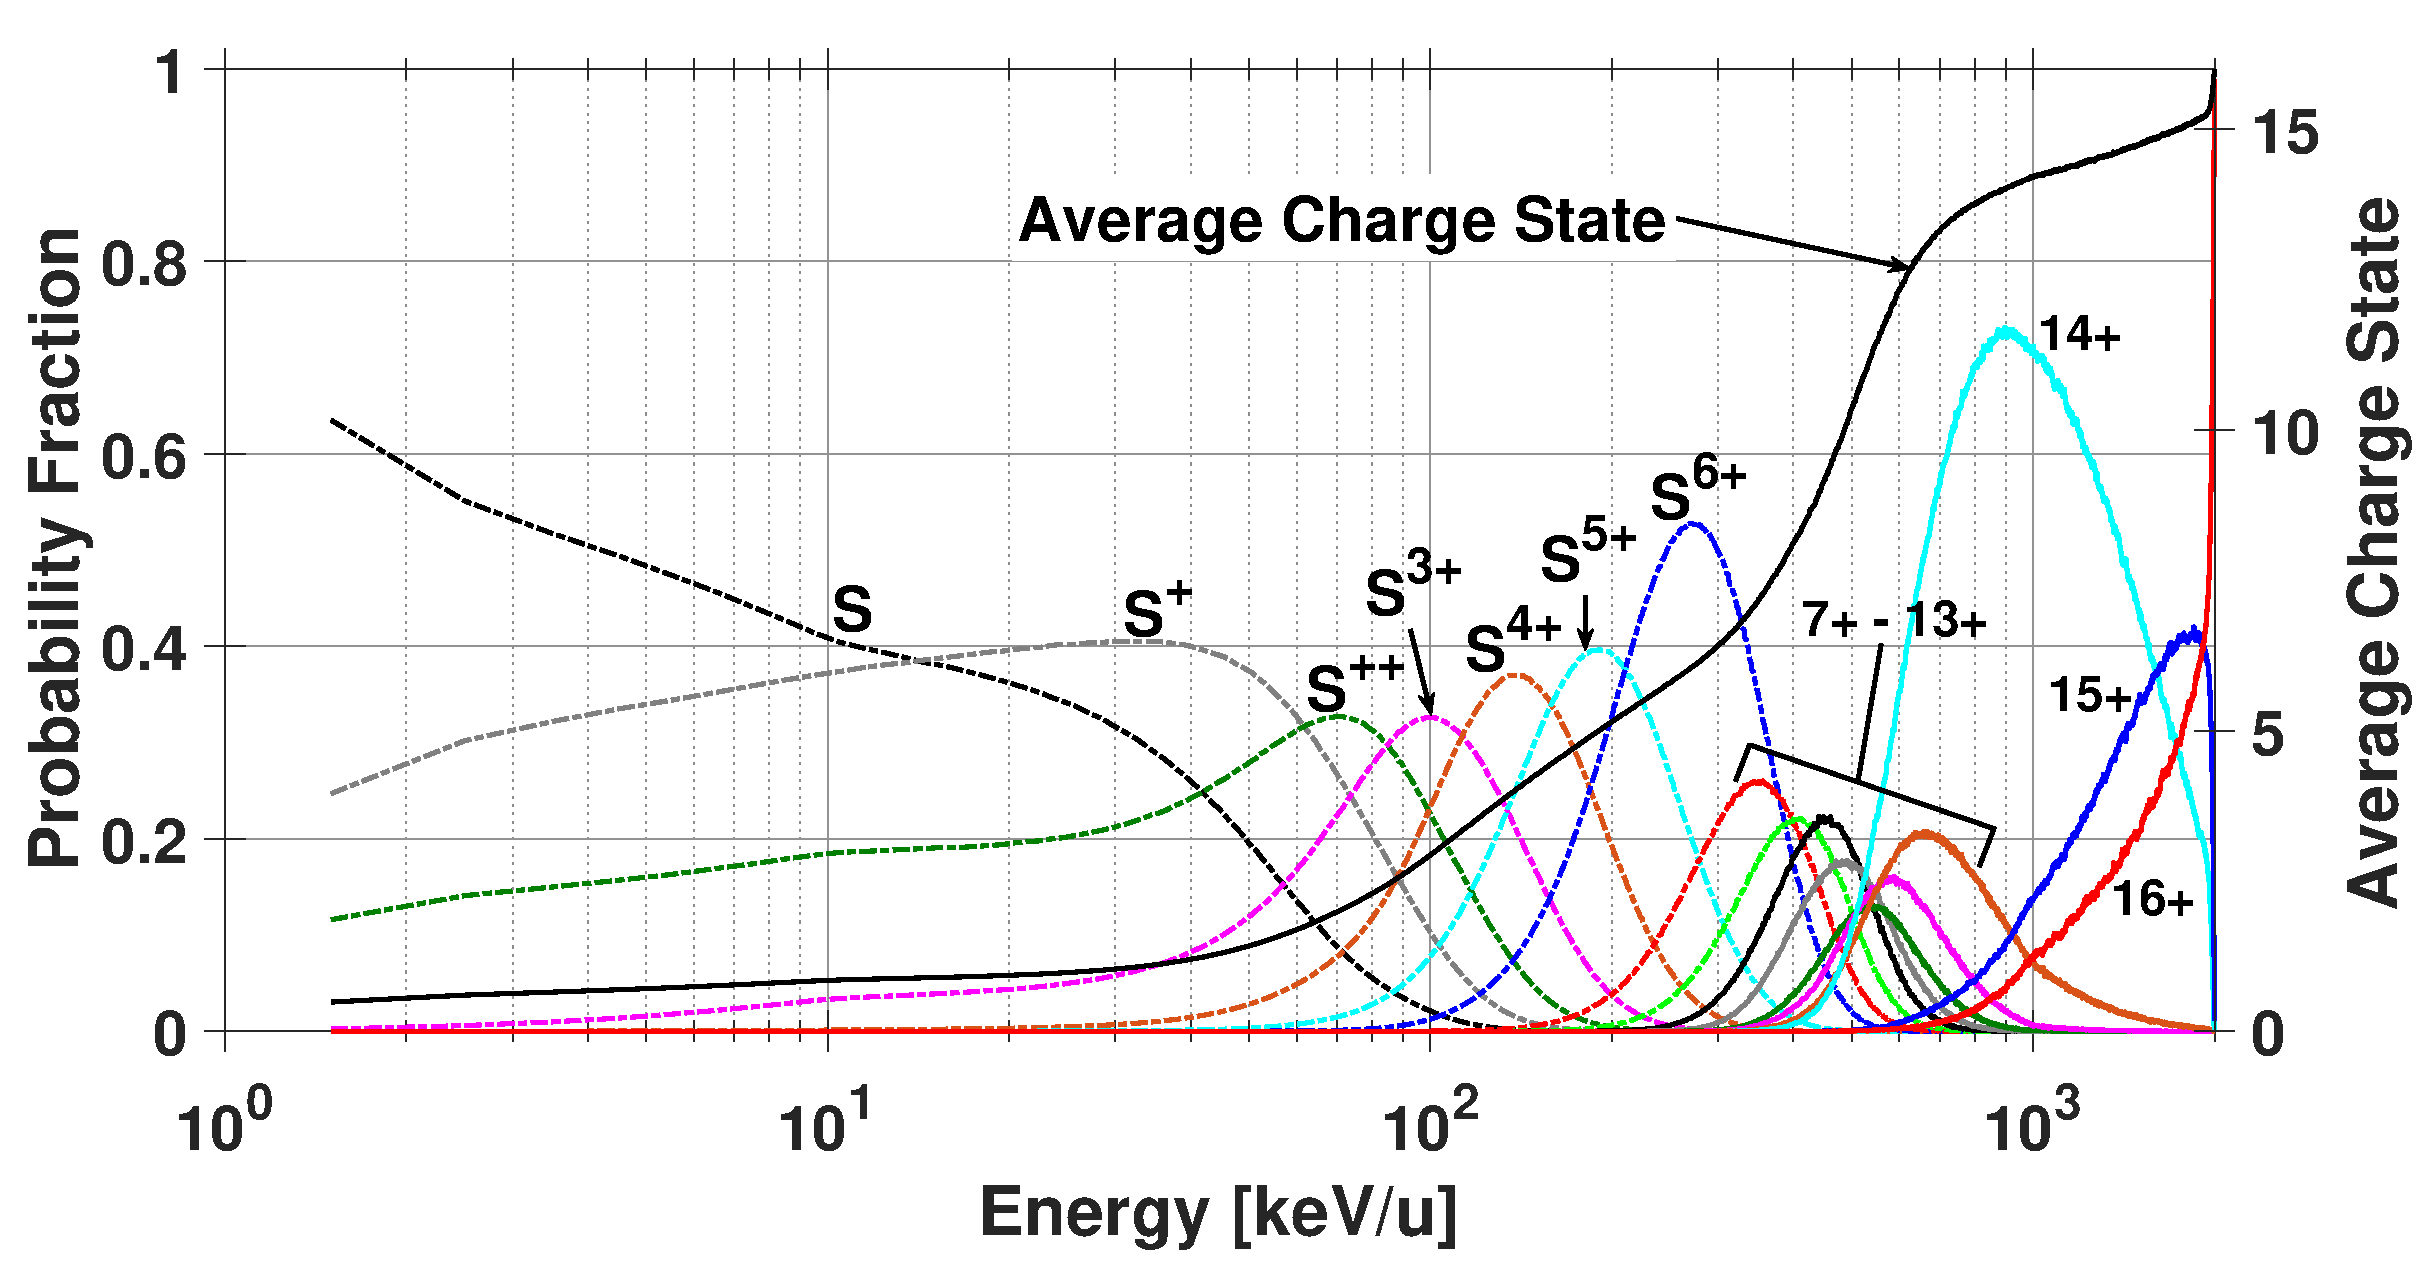
\includegraphics[width=\textwidth]{Figures/CSDsul.eps}
\caption{Sulfur charge state distribution}
\label{fig:CSDsul}
\end{figure}

The charge state equilibrium fractions demonstrate at what energy the ion will reach a given charge state regardless of collision processes undergone or the initial ion energy.
From here, one can see, at a glance, what energies are required for an ion to begin producing X-rays.
For both oxygen and sulfur the sixth charge state must be reached to begin producing X-rays (O$^{6+}$ and S$^{6+}$ with projectile excitation).
These charge states are sufficiently reached for both species at an energy between 100-200 keV/u (a total energy of ~2.4 MeV and ~4.8 MeV for oxygen and sulfur, respectively). 

%  Numbered lines in equations:
%  To add line numbers to lines in equations,
%  \begin{linenomath*}
%  \begin{equation}
%  \end{equation}
%  \end{linenomath*}



%% Enter Figures and Tables near as possible to where they are first mentioned:
%
% DO NOT USE \psfrag or \subfigure commands.
%
% Figure captions go below the figure.
% Table titles go above tables;  other caption information
%  should be placed in last line of the table, using
% \multicolumn2l{$^a$ This is a table note.}
%
%----------------
% EXAMPLE FIGURE
%
% \begin{figure}[h]
% \centering
% when using pdflatex, use pdf file:
% \includegraphics[natwidth=800px,natheight=600px]{figsamp.pdf}
%
% when using dvips, use .eps file:
% \includegraphics[natwidth=800px,natheight=600px]{figsamp.eps}
%
% \caption{Short caption}
% \label{figone}
%  \end{figure}
%
% We recommend that you provide the native width and height (natwidth, natheight) of your figures.
% Specifying native dimensions ensures that your figures are properly scaled
%
%
% ---------------
% EXAMPLE TABLE
%
% \begin{table}
% \caption{Time of the Transition Between Phase 1 and Phase 2$^{a}$}
% \centering
% \begin{tabular}{l c}
% \hline
%  Run  & Time (min)  \\
% \hline
%   $l1$  & 260   \\
%   $l2$  & 300   \\
%   $l3$  & 340   \\
%   $h1$  & 270   \\
%   $h2$  & 250   \\
%   $h3$  & 380   \\
%   $r1$  & 370   \\
%   $r2$  & 390   \\
% \hline
% \multicolumn{2}{l}{$^{a}$Footnote text here.}
% \end{tabular}
% \end{table}

%% SIDEWAYS FIGURE and TABLE
% AGU prefers the use of {sidewaystable} over {landscapetable} as it causes fewer problems.
%
% \begin{sidewaysfigure}
% \includegraphics[width=20pc]{figsamp}
% \caption{caption here}
% \label{newfig}
% \end{sidewaysfigure}
%
%  \begin{sidewaystable}
%  \caption{Caption here}
% \label{tab:signif_gap_clos}
%  \begin{tabular}{ccc}
% one&two&three\\
% four&five&six
%  \end{tabular}
%  \end{sidewaystable}

%% If using numbered lines, please surround equations with \begin{linenomath*}...\end{linenomath*}
%\begin{linenomath*}
%\begin{equation}
%y|{f} \sim g(m, \sigma),
%\end{equation}
%\end{linenomath*}

%%% End of body of article

%%%%%%%%%%%%%%%%%%%%%%%%%%%%%%%%
%% Optional Appendix goes here
%
% The \appendix command resets counters and redefines section heads
%
% After typing \appendix
%
%\section{Here Is Appendix Title}
% will show
% A: Here Is Appendix Title
%
%\appendix
%\section{Here is a sample appendix}

%%%%%%%%%%%%%%%%%%%%%%%%%%%%%%%%%%%%%%%%%%%%%%%%%%%%%%%%%%%%%%%%
%
% Optional Glossary, Notation or Acronym section goes here:
%
%%%%%%%%%%%%%%
% Glossary is only allowed in Reviews of Geophysics
%  \begin{glossary}
%  \term{Term}
%   Term Definition here
%  \term{Term}
%   Term Definition here
%  \term{Term}
%   Term Definition here
%  \end{glossary}

%
%%%%%%%%%%%%%%
% Acronyms
%   \begin{acronyms}
%   \acro{Acronym}
%   Definition here
%   \acro{EMOS}
%   Ensemble model output statistics
%   \acro{ECMWF}
%   Centre for Medium-Range Weather Forecasts
%   \end{acronyms}

%
%%%%%%%%%%%%%%
% Notation
%   \begin{notation}
%   \notation{$a+b$} Notation Definition here
%   \notation{$e=mc^2$}
%   Equation in German-born physicist Albert Einstein's theory of special
%  relativity that showed that the increased relativistic mass ($m$) of a
%  body comes from the energy of motion of the body—that is, its kinetic
%  energy ($E$)—divided by the speed of light squared ($c^2$).
%   \end{notation}




%%%%%%%%%%%%%%%%%%%%%%%%%%%%%%%%%%%%%%%%%%%%%%%%%%%%%%%%%%%%%%%%
%
%  ACKNOWLEDGMENTS
%
% The acknowledgments must list:
%
% >>>>	A statement that indicates to the reader where the data
% 	supporting the conclusions can be obtained (for example, in the
% 	references, tables, supporting information, and other databases).
%
% 	All funding sources related to this work from all authors
%
% 	Any real or perceived financial conflicts of interests for any
%	author
%
% 	Other affiliations for any author that may be perceived as
% 	having a conflict of interest with respect to the results of this
% 	paper.
%
%
% It is also the appropriate place to thank colleagues and other contributors.
% AGU does not normally allow dedications.


\acknowledgments
Enter acknowledgments, including your data availability statement, here.


%% ------------------------------------------------------------------------ %%
%% References and Citations

\bibliography{Biblio/mybiblio}

%%%%%%%%%%%%%%%%%%%%%%%%%%%%%%%%%%%%%%%%%%%%%%%
% BibTeX is preferred:
%
% \bibliography{<name of your .bib file>}
%
% don't specify bibliographystyle
%%%%%%%%%%%%%%%%%%%%%%%%%%%%%%%%%%%%%%%%%%%%%%%



% Please use ONLY \citet and \citep for reference citations.
% DO NOT use other cite commands (e.g., \cite, \citeyear, \nocite, \citealp, etc.).
%% Example \citet and \citep:
%  ...as shown by \citet{Boug10}, \citet{Buiz07}, \citet{Fra10},
%  \citet{Ghel00}, and \citet{Leit74}.

%  ...as shown by \citep{Boug10}, \citep{Buiz07}, \citep{Fra10},
%  \citep{Ghel00, Leit74}.

%  ...has been shown \citep [e.g.,][]{Boug10,Buiz07,Fra10}.


\end{document}



More Information and Advice:

%% ------------------------------------------------------------------------ %%
%
%  SECTION HEADS
%
%% ------------------------------------------------------------------------ %%

% Capitalize the first letter of each word (except for
% prepositions, conjunctions, and articles that are
% three or fewer letters).

% AGU follows standard outline style; therefore, there cannot be a section 1 without
% a section 2, or a section 2.3.1 without a section 2.3.2.
% Please make sure your section numbers are balanced.
% ---------------
% Level 1 head
%
% Use the \section{} command to identify level 1 heads;
% type the appropriate head wording between the curly
% brackets, as shown below.
%
%An example:
%\section{Level 1 Head: Introduction}
%
% ---------------
% Level 2 head
%
% Use the \subsection{} command to identify level 2 heads.
%An example:
%\subsection{Level 2 Head}
%
% ---------------
% Level 3 head
%
% Use the \subsubsection{} command to identify level 3 heads
%An example:
%\subsubsection{Level 3 Head}
%
%---------------
% Level 4 head
%
% Use the \subsubsubsection{} command to identify level 3 heads
% An example:
%\subsubsubsection{Level 4 Head} An example.
%
%% ------------------------------------------------------------------------ %%
%
%  IN-TEXT LISTS
%
%% ------------------------------------------------------------------------ %%
%
% Do not use bulleted lists; enumerated lists are okay.
% \begin{enumerate}
% \item
% \item
% \item
% \end{enumerate}
%
%% ------------------------------------------------------------------------ %%
%
%  EQUATIONS
%
%% ------------------------------------------------------------------------ %%

% Single-line equations are centered.
% Equation arrays will appear left-aligned.

Math coded inside display math mode \[ ...\]
 will not be numbered, e.g.,:
 \[ x^2=y^2 + z^2\]

 Math coded inside \begin{equation} and \end{equation} will
 be automatically numbered, e.g.,:
 \begin{equation}
 x^2=y^2 + z^2
 \end{equation}


% To create multiline equations, use the
% \begin{eqnarray} and \end{eqnarray} environment
% as demonstrated below.
\begin{eqnarray}
  x_{1} & = & (x - x_{0}) \cos \Theta \nonumber \\
        && + (y - y_{0}) \sin \Theta  \nonumber \\
  y_{1} & = & -(x - x_{0}) \sin \Theta \nonumber \\
        && + (y - y_{0}) \cos \Theta.
\end{eqnarray}

%If you don't want an equation number, use the star form:
%\begin{eqnarray*}...\end{eqnarray*}

% Break each line at a sign of operation
% (+, -, etc.) if possible, with the sign of operation
% on the new line.

% Indent second and subsequent lines to align with
% the first character following the equal sign on the
% first line.

% Use an \hspace{} command to insert horizontal space
% into your equation if necessary. Place an appropriate
% unit of measure between the curly braces, e.g.
% \hspace{1in}; you may have to experiment to achieve
% the correct amount of space.


%% ------------------------------------------------------------------------ %%
%
%  EQUATION NUMBERING: COUNTER
%
%% ------------------------------------------------------------------------ %%

% You may change equation numbering by resetting
% the equation counter or by explicitly numbering
% an equation.

% To explicitly number an equation, type \eqnum{}
% (with the desired number between the brackets)
% after the \begin{equation} or \begin{eqnarray}
% command.  The \eqnum{} command will affect only
% the equation it appears with; LaTeX will number
% any equations appearing later in the manuscript
% according to the equation counter.
%

% If you have a multiline equation that needs only
% one equation number, use a \nonumber command in
% front of the double backslashes (\\) as shown in
% the multiline equation above.

% If you are using line numbers, remember to surround
% equations with \begin{linenomath*}...\end{linenomath*}

%  To add line numbers to lines in equations:
%  \begin{linenomath*}
%  \begin{equation}
%  \end{equation}
%  \end{linenomath*}



